%%%%%%%%%%%%%%%%%%%%%%%%%%%%%%%%%%%%%%%%%
% Lachaise Assignment
% LaTeX Template
% Version 1.0 (26/6/2018)
%
% This template originates from:
% http://www.LaTeXTemplates.com
%
% Authors:
% Marion Lachaise & François Févotte
% Vel (vel@LaTeXTemplates.com)
%
% License:
% CC BY-NC-SA 3.0 (http://creativecommons.org/licenses/by-nc-sa/3.0/)
% 
%%%%%%%%%%%%%%%%%%%%%%%%%%%%%%%%%%%%%%%%%

%----------------------------------------------------------------------------------------
%	PACKAGES AND OTHER DOCUMENT CONFIGURATIONS
%----------------------------------------------------------------------------------------

\documentclass[bibnotes]{article}
\usepackage{hyperref}
\usepackage{caption}
\usepackage{subcaption}
\usepackage{mathtools}
\usepackage{natbib}
\usepackage{physics}
\usepackage{amsmath}

% \usepackage{subfig}
%%%%%%%%%%%%%%%%%%%%%%%%%%%%%%%%%%%%%%%%%
% Lachaise Assignment
% Structure Specification File
% Version 1.0 (26/6/2018)
%
% This template originates from:
% http://www.LaTeXTemplates.com
%
% Authors:
% Marion Lachaise & François Févotte
% Vel (vel@LaTeXTemplates.com)
%
% License:
% CC BY-NC-SA 3.0 (http://creativecommons.org/licenses/by-nc-sa/3.0/)
% 
%%%%%%%%%%%%%%%%%%%%%%%%%%%%%%%%%%%%%%%%%

%----------------------------------------------------------------------------------------
%	PACKAGES AND OTHER DOCUMENT CONFIGURATIONS
%----------------------------------------------------------------------------------------

\usepackage{amsmath,amsfonts,stmaryrd,amssymb} % Math packages

\usepackage{enumerate} % Custom item numbers for enumerations

\usepackage[ruled]{algorithm2e} % Algorithms

\usepackage[framemethod=tikz]{mdframed} % Allows defining custom boxed/framed environments

\usepackage{listings} % File listings, with syntax highlighting
\lstset{
	basicstyle=\ttfamily, % Typeset listings in monospace font
}

%----------------------------------------------------------------------------------------
%	DOCUMENT MARGINS
%----------------------------------------------------------------------------------------

\usepackage{geometry} % Required for adjusting page dimensions and margins

\geometry{
	paper=a4paper, % Paper size, change to letterpaper for US letter size
	top=2.5cm, % Top margin
	bottom=3cm, % Bottom margin
	left=2.5cm, % Left margin
	right=2.5cm, % Right margin
	headheight=14pt, % Header height
	footskip=1.5cm, % Space from the bottom margin to the baseline of the footer
	headsep=1.2cm, % Space from the top margin to the baseline of the header
	%showframe, % Uncomment to show how the type block is set on the page
}

%----------------------------------------------------------------------------------------
%	FONTS
%----------------------------------------------------------------------------------------

\usepackage[utf8]{inputenc} % Required for inputting international characters
\usepackage[T1]{fontenc} % Output font encoding for international characters

\usepackage{XCharter} % Use the XCharter fonts

%----------------------------------------------------------------------------------------
%	COMMAND LINE ENVIRONMENT
%----------------------------------------------------------------------------------------

% Usage:
% \begin{commandline}
%	\begin{verbatim}
%		$ ls
%		
%		Applications	Desktop	...
%	\end{verbatim}
% \end{commandline}

\mdfdefinestyle{commandline}{
	leftmargin=10pt,
	rightmargin=10pt,
	innerleftmargin=15pt,
	middlelinecolor=black!50!white,
	middlelinewidth=2pt,
	frametitlerule=false,
	backgroundcolor=black!5!white,
	frametitle={Command Line},
	frametitlefont={\normalfont\sffamily\color{white}\hspace{-1em}},
	frametitlebackgroundcolor=black!50!white,
	nobreak,
}

% Define a custom environment for command-line snapshots
\newenvironment{commandline}{
	\medskip
	\begin{mdframed}[style=commandline]
}{
	\end{mdframed}
	\medskip
}

%----------------------------------------------------------------------------------------
%	FILE CONTENTS ENVIRONMENT
%----------------------------------------------------------------------------------------

% Usage:
% \begin{file}[optional filename, defaults to "File"]
%	File contents, for example, with a listings environment
% \end{file}

\mdfdefinestyle{file}{
	innertopmargin=1.6\baselineskip,
	innerbottommargin=0.8\baselineskip,
	topline=false, bottomline=false,
	leftline=false, rightline=false,
	leftmargin=2cm,
	rightmargin=2cm,
	singleextra={%
		\draw[fill=black!10!white](P)++(0,-1.2em)rectangle(P-|O);
		\node[anchor=north west]
		at(P-|O){\ttfamily\mdfilename};
		%
		\def\l{3em}
		\draw(O-|P)++(-\l,0)--++(\l,\l)--(P)--(P-|O)--(O)--cycle;
		\draw(O-|P)++(-\l,0)--++(0,\l)--++(\l,0);
	},
	nobreak,
}

% Define a custom environment for file contents
\newenvironment{file}[1][File]{ % Set the default filename to "File"
	\medskip
	\newcommand{\mdfilename}{#1}
	\begin{mdframed}[style=file]
}{
	\end{mdframed}
	\medskip
}

%----------------------------------------------------------------------------------------
%	NUMBERED QUESTIONS ENVIRONMENT
%----------------------------------------------------------------------------------------

% Usage:
% \begin{question}[optional title]
%	Question contents
% \end{question}

\mdfdefinestyle{question}{
	innertopmargin=1.2\baselineskip,
	innerbottommargin=0.8\baselineskip,
	roundcorner=5pt,
	nobreak,
	singleextra={%
		\draw(P-|O)node[xshift=1em,anchor=west,fill=white,draw,rounded corners=5pt]{%
		\questionTitle};
	},
}

%\newcounter{Question} % Stores the current question number that gets iterated with each new question

% Define a custom environment for numbered questions
\newenvironment{question}[1][\unskip]{
	\bigskip
%	\stepcounter{Question}
	\newcommand{\questionTitle}{~#1}
	\begin{mdframed}[style=question]
}{
	\end{mdframed}
	\medskip
}

%----------------------------------------------------------------------------------------
%	WARNING TEXT ENVIRONMENT
%----------------------------------------------------------------------------------------

% Usage:
% \begin{warn}[optional title, defaults to "Warning:"]
%	Contents
% \end{warn}

\mdfdefinestyle{warning}{
	topline=false, bottomline=false,
	leftline=false, rightline=false,
	nobreak,
	singleextra={%
		\draw(P-|O)++(-0.5em,0)node(tmp1){};
		\draw(P-|O)++(0.5em,0)node(tmp2){};
		\fill[black,rotate around={45:(P-|O)}](tmp1)rectangle(tmp2);
		\node at(P-|O){\color{white}\scriptsize\bf !};
		\draw[very thick](P-|O)++(0,-1em)--(O);%--(O-|P);
	}
}

% Define a custom environment for warning text
\newenvironment{warn}[1][Warning:]{ % Set the default warning to "Warning:"
	\medskip
	\begin{mdframed}[style=warning]
		\noindent{\textbf{#1}}
}{
	\end{mdframed}
}

%----------------------------------------------------------------------------------------
%	INFORMATION ENVIRONMENT
%----------------------------------------------------------------------------------------

% Usage:
% \begin{info}[optional title, defaults to "Info:"]
% 	contents
% 	\end{info}

\mdfdefinestyle{info}{%
	topline=false, bottomline=false,
	leftline=false, rightline=false,
	nobreak,
	singleextra={%
		\fill[black](P-|O)circle[radius=0.4em];
		\node at(P-|O){\color{white}\scriptsize\bf i};
		\draw[very thick](P-|O)++(0,-0.8em)--(O);%--(O-|P);
	}
}

% Define a custom environment for information
\newenvironment{info}[1][Note:]{ % Set the default title to "Info:"
	\medskip
	\begin{mdframed}[style=info]
		\noindent{\textbf{#1}}
}{
	\end{mdframed}
}
 % Include the file specifying the document structure and custom commands

%----------------------------------------------------------------------------------------
%	ASSIGNMENT INFORMATION
%----------------------------------------------------------------------------------------

\newcommand{\SLJ}[3]{{\ensuremath{{^{#1}}\mathrm{#2}_{#3}}}}
\newcommand{\TPT}{\SLJ{3}{P}{2}}
\newcommand{\TPO}{\SLJ{3}{P}{1}}
\newcommand{\TPZ}{\SLJ{3}{P}{0} \ }
\newcommand{\TPJ}{\SLJ{3}{P}{J}}
\newcommand{\TSO}{\SLJ{3}{S}{1}}
\newcommand{\SSZ}{\SLJ{1}{S}{0} \ }
\newcommand{\SPO}{\SLJ{1}{P}{1}}
\newcommand{\TDO}{\SLJ{3}{D}{1}}
\newcommand{\SDT}{\SLJ{1}{D}{2}}


\title{Cavity Ring Project Data Analysis} % Title of the assignment

\author{Annie Jihyun Park\\ \texttt{ajpark@mpq.mpg.de}} % Author name and email address

\date{\today} % University, school and/or department name(s) and a date

%----------------------------------------------------------------------------------------

\begin{document}

\maketitle % Print the title

%----------------------------------------------------------------------------------------
%	INTRODUCTION
%----------------------------------------------------------------------------------------

\section*{Introduction} % Unnumbered section

	We use the spatially dependent ac-stark shift on the clock transition to map the intensity profile of the cavity lattices. This document summarizes the data analysis went into the cavity fringe project. 

% The focus of our paper will be about integrating the build-up cavities for optical lattice experiments, demonstrating its viability to create high contrast, large, homogeneous, and deep optical lattices in a stable and compact way.
% The Gaussian intensity profile of optical lattices is one of the central features that characterizes the homogeneity and size of the lattices. For this reason, 
% For this reason, we chose the lattice wavelength to be 914 nm to maximize the stark shift, whereas the sheet beam wavelength is magic, 813 nm, to eliminate the influence of the sheet light. 
%----------------------------------------------------------------------------------------
%	PROBLEM 1
%----------------------------------------------------------------------------------------
\tableofcontents

\section{Potential}

	\begin{figure}[h]
	    \centering
	    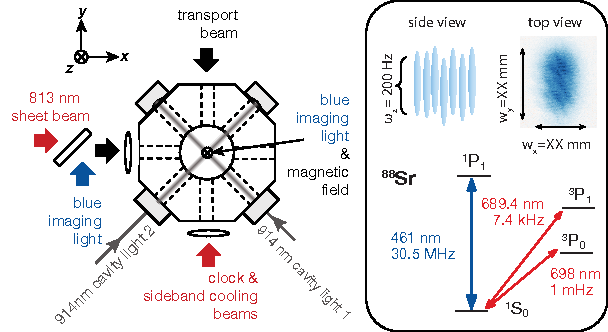
\includegraphics[]{figures/setup.pdf}
	    \caption{Optical setup}
	    \label{fig:setup}
	\end{figure}

	The optical trap is generated by the two-dimensional optical lattices created in the build-up cavity and a sheet-like dipole trap, as illustrated in Figure \ref{fig:setup}. Since the sheet beam is magic to the clock transition and its trap frequency is much smaller than the lattice trap frequencies ($\sim$ 200 Hz), we ignore the influence of the sheet beam for now. For the two-dimensional lattices, the potential is

	\begin{align}
	U(x,y,z)&=U^{x}_{0}\bigg(\frac{w_{0}}{w(x)}\bigg)^{2}e^{-2(y^{2}+z^{2})/w^{2}_{0}}\text{cos}^{2}(kx)+U^{y}_{0}\bigg(\frac{w_{0}}{w(y)}\bigg)^{2}e^{-2(x^{2}+z^{2})/w^{2}_{0}}\text{cos}^{2}(ky) \nonumber \\
	&\stackrel{x,y \approx 0}{\approx} U^{x}_{0}e^{-2(y^{2}+z^{2})/w^{2}_{0}}\text{cos}^{2}(kx)+U^{y}_{0}e^{-2(x^{2}+z^{2})/w^{2}_{0}}\text{cos}^{2}(ky) \nonumber\\
	&\stackrel{U_{x}=U_{y}, z\approx{0}}{\approx} U_{0}\bigg(e^{-2y^{2}/w^{2}_{0}}\text{cos}^{2}(kx)+e^{-2x^{2}/w^{2}_{0}}\text{cos}^{2}(ky)\bigg),
	\label{eq:2d_potential}
	\end{align}

	\noindent where $U^{i}_{0} = - \alpha I_{0} / (2c\epsilon_{0})$ where $\alpha$ is polarizability, and $w_{0}$ is the waist of the cavity mode. In Equation \ref{eq:2d_potential}, we made two approximations $w_{0}/w(x)\approx1$ and $e^{-2z^{2}/w^{2}_{0}}\approx 1$, which are valid because the rayleigh range of the cavities modes are $\sim 70$ cm and the sheet confines the atoms at the gravity compensated position $z\approx 60 \ \mu \text{m} \ll  w_{0}$. The vibrational energy of atoms trapped in the deep two-dimensional optical lattices ~\cite{blatt09} is (or by solving the Mathieu equation as in the Sebastian's ring simulation code)

	\begin{align}\label{eq:2d_potential_vmode_energy}
	E_{n_x,n_y}&=h\nu_{x}(n_{x}+1/2)-h\frac{\nu_{\text{rec}}}{2}(n^{2}_{x}+n_{x}+1)
	+h\nu_{y}(n_{y}+1/2)-h\frac{\nu_{\text{rec}}}{2}(n^{2}_{y}+n_{y}+1) \nonumber\\
	&\stackrel{\nu_x=\nu_y}=h\nu + n_{xy}h\nu - h\frac{\nu_{\text{rec}}}{2}(n^{2}_x+n^{2}_y+n+2)
	\end{align}

	\noindent where $n_{i}$, $\nu_{\text{rec}}$, and $n_{xy}$ are vibrational mode along $i$ axis, recoil frequency, and $n_x+n_y$, respectively. Following Equation \ref{eq:2d_potential_vmode_energy}, the energies of $n_{00}=0$ or $n_{10}=1$ (or $n_{01}$) states are

	\begin{align}
	\begin{split}\label{eq:energy_deep_lattice_n0}
		& E_{0,0}=h\nu-h\nu_{\text{rec}}
	\end{split}\\
	\begin{split}\label{eq:energy_deep_lattice_n1}
		& E_{1,0}=2h\nu-2h\nu_{\text{rec}}
	\end{split}\\
	& \Delta E = h(\nu - \nu_{\text{rec}})\nonumber.
	% \label{eq:energy_deep_lattice}
	\end{align}


	\noindent So far, all the discussions have been the energies of a particular state in the trap. Now, let's look at the detuning required to drive the ground to excited states in the trap as illustrated in Figure \ref{fig:potential_intro}. This is particularly important for our purposes, since we are using this technique to characterize the cavity lattices. Since we are in non-magic lattices, we need to remember that the trap frequencies are different for the two states.

	\begin{figure}
	    \centering
	    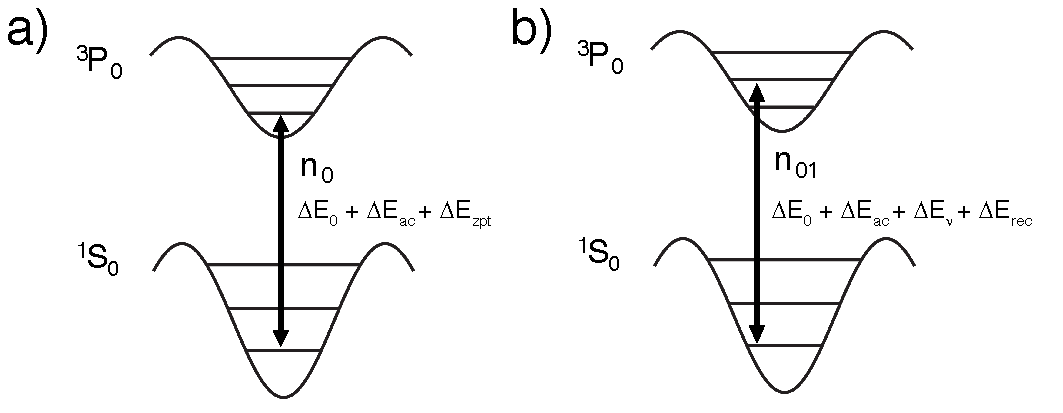
\includegraphics[scale=0.8]{figures/potential_intro.pdf}
	    \caption{Energy required to drive carrier and sideband transitions}
	    \label{fig:potential_intro}
	\end{figure}


	In free space, the energy difference between $\SSZ (g)$ and $\TPZ (e)$ states are given by $\Delta E_{0}=\hbar\omega_{0}$. In non-magic lattices, there are additional shifts to consider: ac-Stark shift ($\Delta E_{\text{ac}}$) and a shift due to vibrational mode energy difference ($\Delta E_\nu$). Let's first consider the energy required to drive a carrier transition $n^{g}_{00}\xleftrightarrow{}n^{e}_{00}$ (Figure \ref{fig:potential_intro}), where $n^{i}_{jk}$ specifies vibrational mode $jk$ of a state $i$, 

	\begin{align}
	\Delta E&=\Delta E_{0}+\Delta E_{\text{ac}} + \Delta E_{\nu} \nonumber\\ 
	&=\hbar\omega_0+ \frac{I(x,y)}{c\epsilon_0}(\alpha_g-\alpha_e)+h(\nu_e-\nu_g) \nonumber \nonumber\\
	&\approx\hbar\omega_0+ \frac{I(x,y)}{c\epsilon_0}(\alpha_g-\alpha_e)+
	\sqrt{\frac{2h\nu_{\text{rec}}I(x,y)}{c\epsilon_{0}}}(\sqrt{\alpha_e}-\sqrt{\alpha_g}),
	\label{eq:carrier_energy}
	\end{align}

	\noindent where $\alpha_{i}$ and $\nu_{i}$ are the polarizability and trap frequency of a state $i$, respectively. To calculate $\Delta E_{\nu}$, we use Equation \ref{eq:energy_deep_lattice_n0}. In the last step, we use $\nu_{\text{i}}\approx 2\sqrt{\nu_{\text{rec}}\abs{U_{i}}/h}$ where $U_{i}=-\alpha_{i}I(x,y)/2c\epsilon_0$, assuming the lattices with perfect contrasts. Rewriting Equation \ref{eq:carrier_energy}, the detuning required to drive a $n^{g}_{00}$ to $n^{e}_{00}$ is 

	% \begin{align*}
	% \delta&=\frac{I(x,y)}{2c\epsilon_0}(\alpha_g-\alpha_e)+h(\nu_e-\nu_g) \nonumber\\
	% &\approx \frac{I(x,y)}{2c\epsilon_0h}(\alpha_g-\alpha_e)+\sqrt{\frac{2\nu_{\text{rec}}I(x,y)}{c\epsilon_{0}h}}(\sqrt{\alpha_e}-\sqrt{\alpha_g}),\\
	% % \label{eq:detuning}
	% \end{align*}

	\begin{align}
	\delta&=\frac{\nu^{2}_g}{2\nu_{\text{rec}}}\bigg(1-\frac{\alpha_e}{\alpha_g}\bigg) + \nu_g\bigg(\sqrt{\frac{\alpha_e}{\alpha_g}}-1\bigg)
	\label{eq:carrier_freq_vg}
	\end{align}

	\noindent or writing in terms of $\nu_e$ instead, one arrives at 

	\begin{align}
	\delta&=\frac{\nu^{2}_e}{2\nu_{\text{rec}}}\bigg(\frac{\alpha_g}{\alpha_e}-1\bigg) + \nu_e\bigg(1-\sqrt{\frac{\alpha_g}{\alpha_e}}\bigg).
	\label{eq:carrier_freq_ve}
	\end{align}


	\noindent We can also look at $\Delta E$ required to drive a sideband transition $n^{g}_{ii} \xleftrightarrow{} n^{e}_{i,i+1}$


	\begin{align}
	\Delta E&=\Delta E_{0}+\Delta E_{\text{ac}} + \Delta E_{\nu} \nonumber \\ 
	&=\hbar\omega_0+ \frac{I(x,y)}{c\epsilon_0}(\alpha_g-\alpha_e)+h(\nu_e-\nu_{\text{rec}}) \nonumber \\
	&\approx\hbar\omega_0+ \frac{I(x,y)}{c\epsilon_0}(\alpha_g-\alpha_e)+h\bigg(\sqrt{\frac{2\nu_{\text{rec}}I(x,y)}{c\epsilon_0 h}}-\nu_{\text{rec}}\bigg),
	% \label{eq:sideband_energy}
	\end{align}

	\noindent where, again, the perfect contrast lattice assumption has been made in the last step. 

	% The maximum trap depth is 2$\abs{U_{0}}$ where $U_{0}=-\alpha_{\SSZ}I(0,0)/2c\epsilon_0$, and the maximum differential trap depth is 

	% \begin{align*}
	% \delta U_{\text{max}}=2U_{0}\bigg(1-\frac{\alpha_{e}}{\alpha_{g}}\bigg).
	% \end{align*}

	% \noindent For the perfect contrast lattices, one can get write $U_{\text{max}}$ in terms of $\nu_{g}$ and polarizability ratio $\alpha_g/\alpha_e$

	% \begin{align}
	% \delta U_{\text{max}}=2\bigg(\frac{h\nu^{2}_{g}}{4\nu_{\text{rec}}}\bigg)\bigg(1-\frac{\alpha_{e}}{\alpha_{g}}\bigg).
	% \end{align}


	% The energy required to drive a carrier transition ($n_{i,i}^{\SSZ} \xleftrightarrow{} n_{i,i}^{\TPZ}$ where $n^{k}_{i,j}$ indicates motional state $i,j$ of the state $k$$) is

	% \begin{align*}
 % 	\Delta E &= \Delta E_{0} + \Delta E_{\text{ac}} + \Delta E_{\text{zpt}}, \\
	% & = \hbar \omega_{0},
	% \end{align*}

	% \noindent where $E_{0}$, 

\section{Measurements}
	\subsection{Gaussian intensity profile}
	\subsection{Ground and excited state trap frequencies ($\alpha_{\text{g}}/\alpha_{\text{e}}$)}

		In two-dimensional non-magic lattices for \SSZ (g) and \TPZ (e) states, the carrier transitions are resolved. As illustrated in Figure \ref{fig:trap_frequency_schematics}, by subtracting the carrier ($n^{g}_{00}\xleftrightarrow{} n^{e}_{00}$ or $n^{g}_{11}\xleftrightarrow{} n^{g}_{11}$) and blue sideband ($n^{g}_{00}\xleftrightarrow{} n^{e}_{10}$) transition frequencies, we can find ground and excited state trap frequencies. This can be easily derived from Equation \ref{eq:energy_deep_lattice_n0} and \ref{eq:energy_deep_lattice_n1}

		\begin{figure}
		    \centering
		    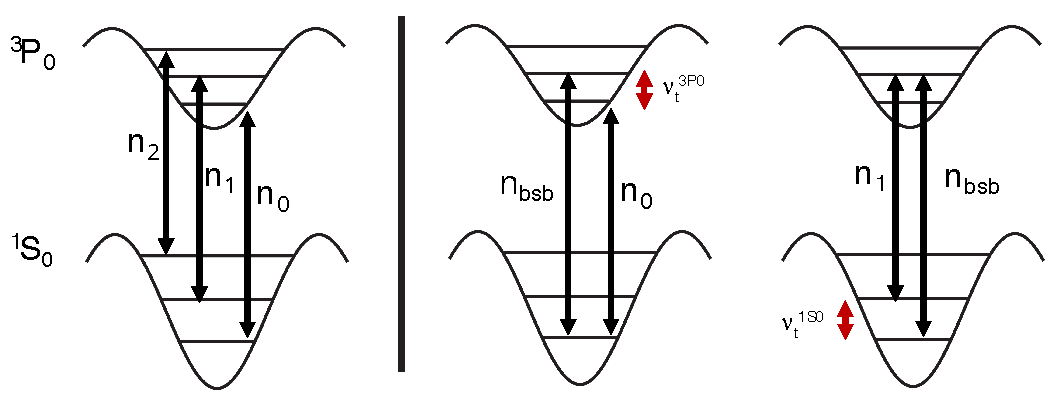
\includegraphics[scale=0.8]{figures/trap_frequency_schematics.pdf}
		    \caption{Carrier transitions are resolved (left) and by combining carrier and sideband transitions, one can find out ground and excited trap frequencies (right two pictures)}
		    \label{fig:trap_frequency_schematics}
		\end{figure}

			\begin{align*}
				\Delta f_{00,10}-\Delta f_{00,00}&=(E^{e}_{1,0}-E^{g}_{0,0})/h-(E^{e}_{0,0}-E^{g}_{0,0})/h \\
				&=(2\nu_e-2\nu_{\text{rec}}-\nu_g+\nu_{\text{rec}})-(\nu_e-\nu_{\text{rec}}-\nu_g+\nu_{\text{rec}}) \\		
				&=(2\nu_e-\nu_g-\nu_{\text{rec}})-(\nu_e-\nu_g) \\	
				&=\nu_e-\nu_{\text{rec}}
			\end{align*}
		and
			\begin{align*}
				\Delta f_{00,10}-\Delta f_{11,11}&=(E^{e}_{1,0}-E^{g}_{0,0})/h-(E^{e}_{1,0}-E^{g}_{1,0})/h \\
				&=(2\nu_e-2\nu_{\text{rec}}-\nu_g+\nu_{\text{rec}})-(2\nu_e-2\nu_{\text{rec}}-2\nu_g+2\nu_{\text{rec}}) \\		
				&=(2\nu_e-\nu_g)-(2\nu_e-2\nu_g) \\	
				&=\nu_g-\nu_{\text{rec}},
			\end{align*}

		\noindent where $f_{ij,kf}$ is the transition frequency from $n^{g}_{ij}\xleftrightarrow{} n^{g}_{kf}$.
		Figure \ref{fig:carrier_sideband_spectra} shows the carrier and sideband spectra for 2 by 2 averaged pixels. From the Lorentzian fits, we can find out $\Delta f_{00,00}$, $\Delta f_{11,11}$, and $\Delta f_{00,10}$. By subtracting the correct pairs, we can find out the polarizability ratio

		\begin{align*}
			&\frac{\alpha_g}{\alpha_e}=\bigg(\frac{\Delta f_{00,10}-\Delta f_{11,11}+\nu_{\text{rec}}}{\Delta f_{00,10}-\Delta f_{00,00}+\nu_{\text{rec}}}\bigg)^{2}
		\end{align*}

		 The result is shown on the left in Figure \label{fig:pol_ratio}, which clearly depicts that our estimation is susceptible to systemic errors. Ideally one would expect a flat distribution of the ratio across the sample; however, we see the ratio gets high as we go further away from the central pixel. So far, we are not sure what the cause is. If we ignore this systemic effect and restrict the estimation in a smaller central region (left on Figure \label{fig:pol_ratio}), the noise distribution seems random. In this central area, the estimated ratio is \textbf{1.179 $\pmb{\pm}$ 0.002}. 

		\begin{figure}
		    \centering
		    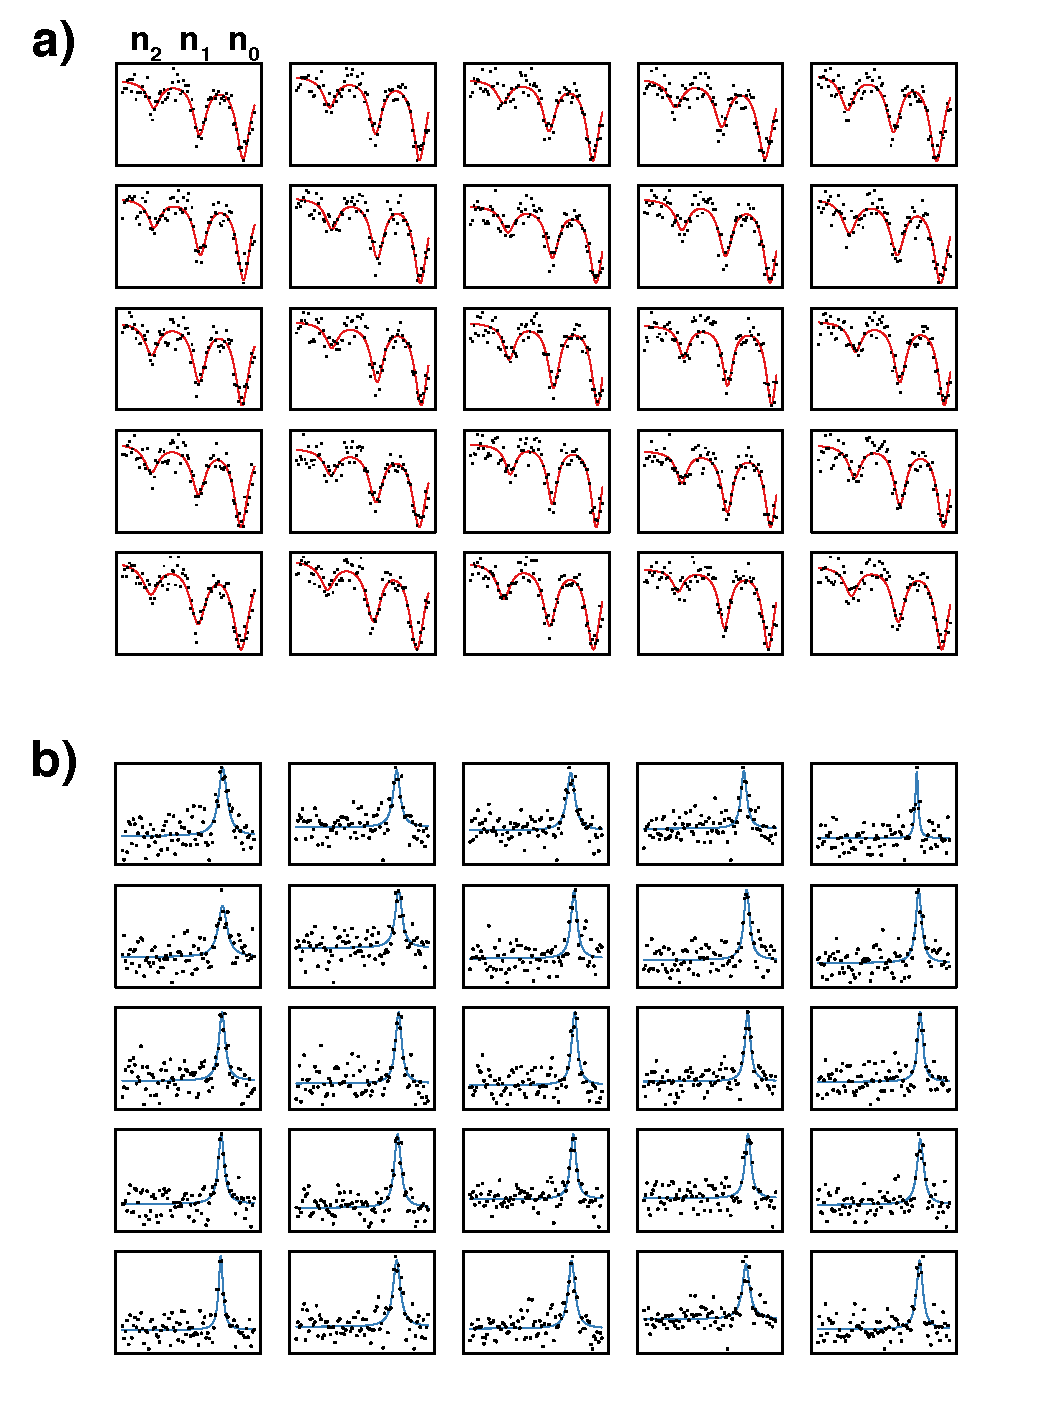
\includegraphics[scale=0.8]{figures/carrier_sideband_spectra.pdf}
		    \caption{Carrier sideband spectra, data folder: \textbackslash data \textbackslash\_2020\textbackslash10\textbackslash29\textbackslash it\_sr88\_clock\_fringe\\ \_arm1=1.175V\_arm2\_0.975V\_z\_cooling\_2 \& it\_sr88\_clock\_fringe\_arm1=1.175V\_arm2\_0.975V\_bluesideband\_fine}
		    \label{fig:carrier_sideband_spectra}
		\end{figure}

		\begin{figure}
		% \centering 
		\hspace*{-2cm}
		\label{fig:pol_ratio}
		\begin{subfigure}{0.4\linewidth}
			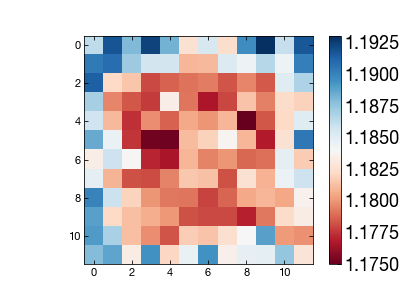
\includegraphics[scale=0.7]{figures/pol_ratio_size6.png}
			% \caption{}
		\end{subfigure}
		\qquad\qquad\qquad\quad
		\begin{subfigure}{0.4\linewidth}
			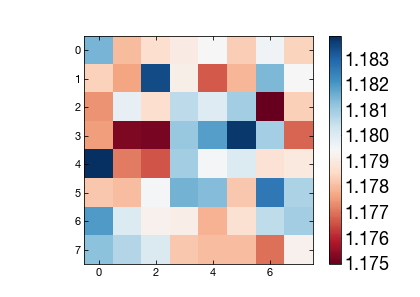
\includegraphics[scale=0.7]{figures/pol_ratio_size4.png}
			% \caption{}
		\end{subfigure}
		\caption{Polarizability $\alpha_g/\alpha_e$ ratio for (a) larger size (b) smaller size} 
		\end{figure}


	\subsection{Absolute clocklaser detuning}
			We measure the absolute clocklaser detuning required to address the atoms in the center of the lattices by beating the frequency comb with the clock laser. The expected detuning as a function of trap frequency (intensity) is described in Equation \ref{eq:carrier_freq_vg} and \ref{eq:carrier_freq_ve} (Equation \ref{eq:carrier_energy}). The clock laser is splitted into multiple paths as shown in Figure \ref{fig:clocklaser setup}, one of the paths is fiber coupled to the frequency comb setup, and the other path goes through a scanning double pass (DP) aom and fiber coupled to seed the injection, which is used to probe the atomic cloud. 

		\begin{figure}
		    \centering
		    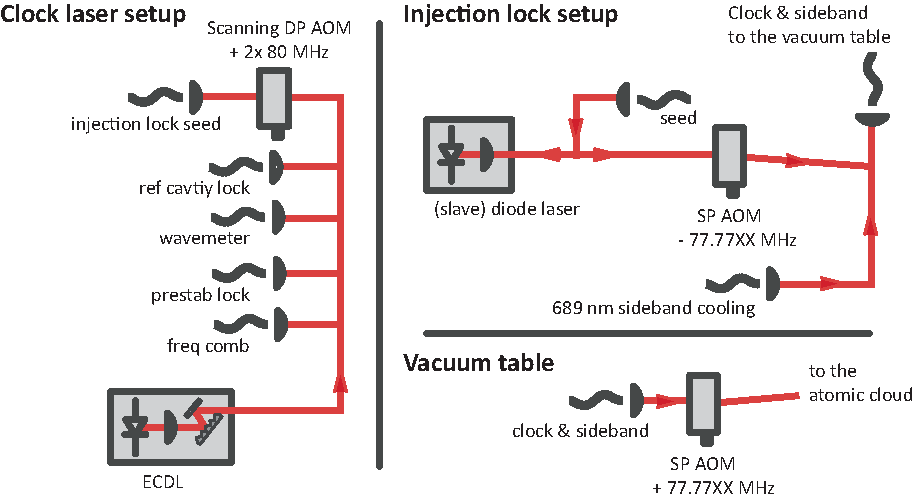
\includegraphics[scale=0.8]{figures/clocklaser_setup.pdf}
		    \caption{Clocklaser setup}
		    \label{fig:clocklaser setup}
		\end{figure}

			To measure the maximum light shift, we scanned the double pass aom frequency to excite the center of the atoms with the clock excitation. We repeated this measurements for two different trap frequencies. Figure \ref{fig:total_ac_stark_spectrum} shows the carrier and blue sideband spectra. Taking each spectrum takes about half an hour to an hour, and after each carrier scan, we recorded the beat frequency recorded on the counter to find out the absolute ac-Stark shift.

			The detunings with respect to the known $^{\text{88}}{\text{Sr}}$ \SSZ - \TPZ transition frequency~\cite{sansonetti10} were,


			\begin{itemize}
			  \item (399533 $\pm$ 400) Hz for "high depth"
			  \item (195385 $\pm$ 400) Hz for "half depth"
			\end{itemize}


			We know that the clock laser drift about -400 Hz per hour. During the carrier frequency measurements, the DP aom frequeny has been compensating for the drift, whereas the fiber port that was used for the beat does not go through this DP aom, thus, susceptible for the drift. If we include this shift, 

			\begin{itemize}
			  \item (399533 $\pm$ 400 + 400) Hz for "high depth"
			  \item (195385 $\pm$ 400 + 400) Hz for "half depth"
			\end{itemize}

		% \begin{figure*}
		% \centering 
		% 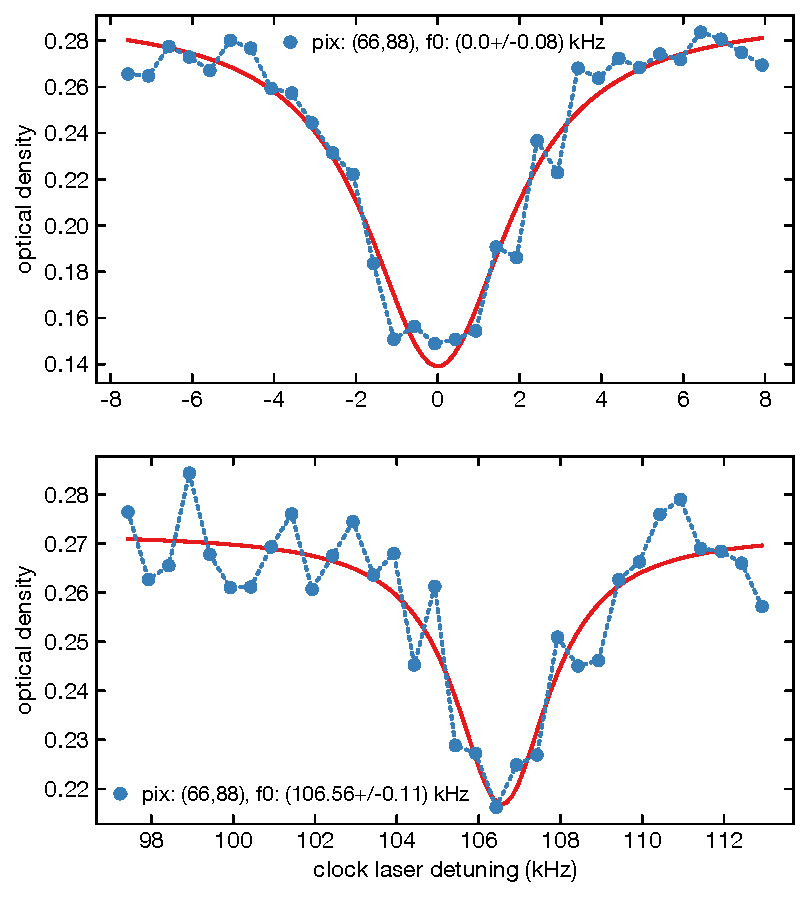
\includegraphics[scale=0.5]{figures/high_depth66_88.pdf}\qquad\quad
		% 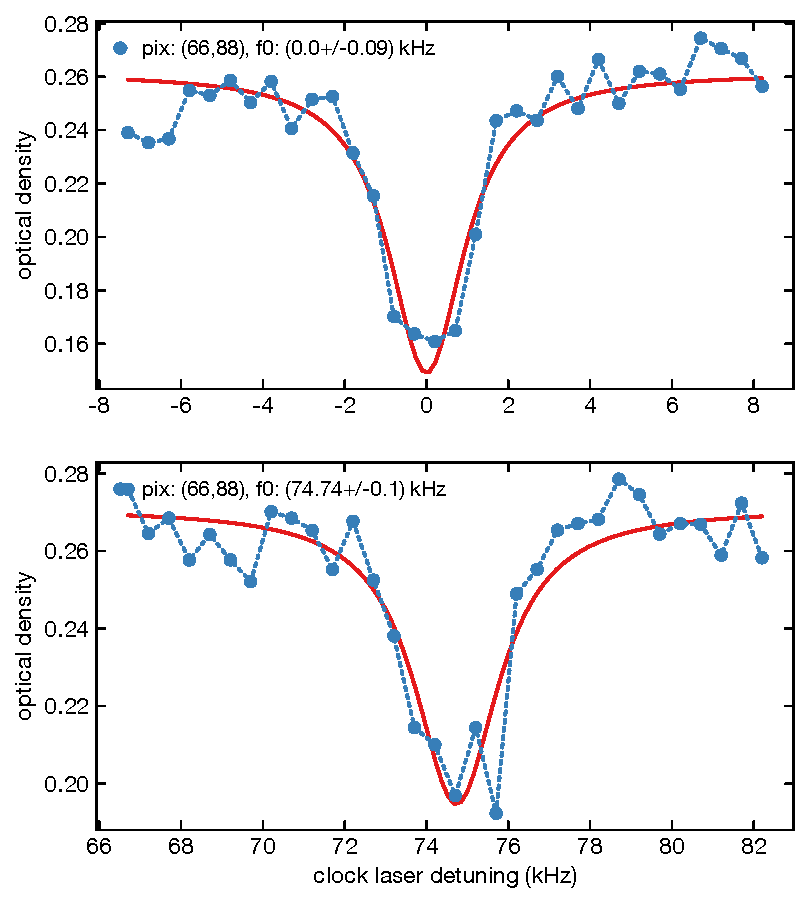
\includegraphics[scale=0.5]{figures/half_depth66_88.pdf}\par\medskip
		% 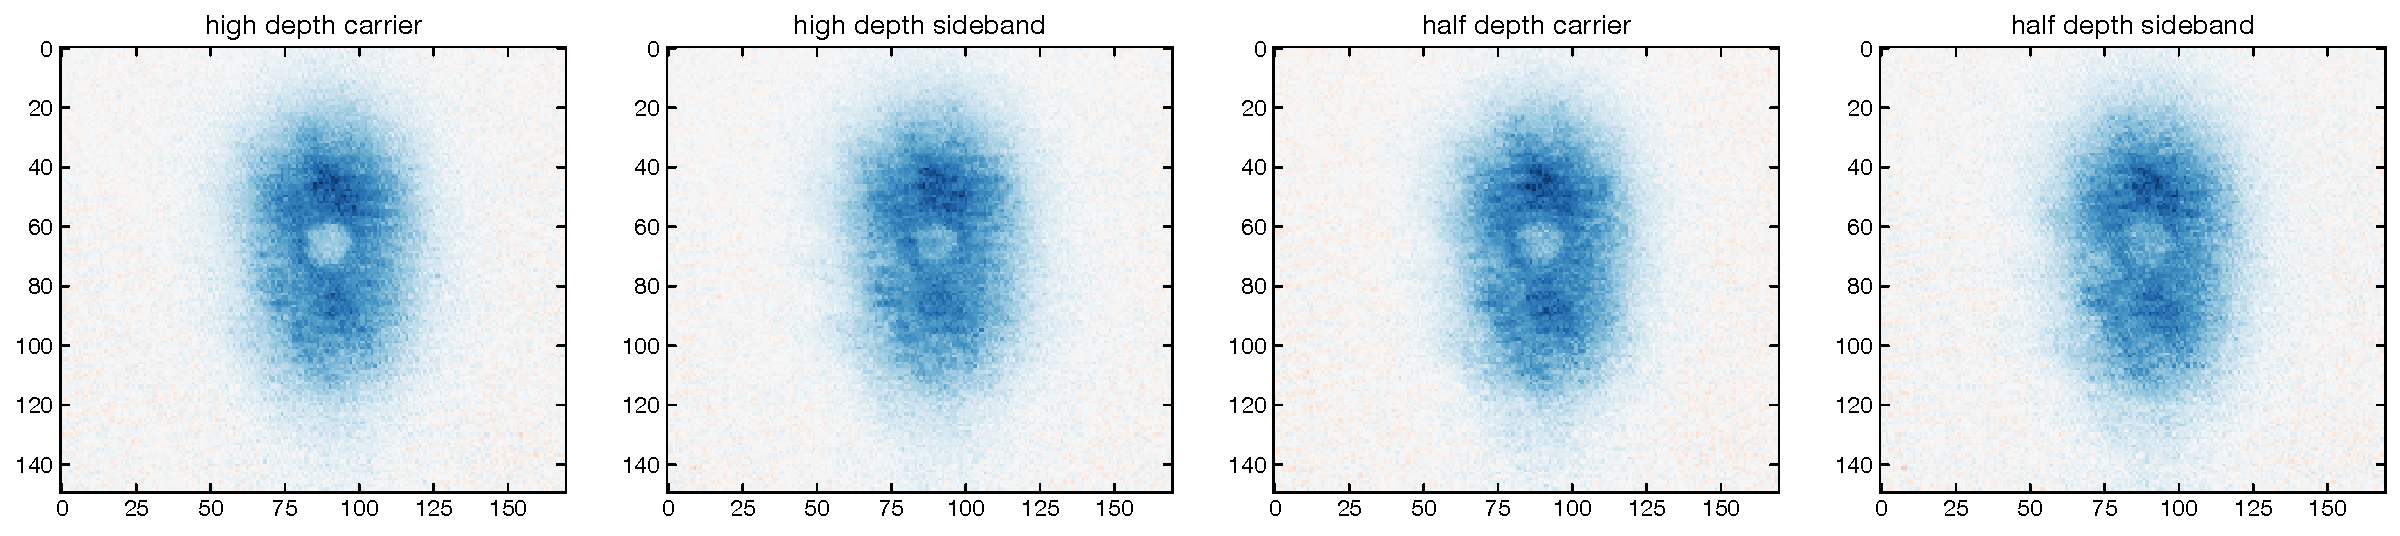
\includegraphics[width=\textwidth]{figures/insitu_images.pdf}
		% \caption{}
		% \end{figure*}

			\begin{figure}
			\centering 
			\begin{subfigure}[b]{0.4\linewidth}
				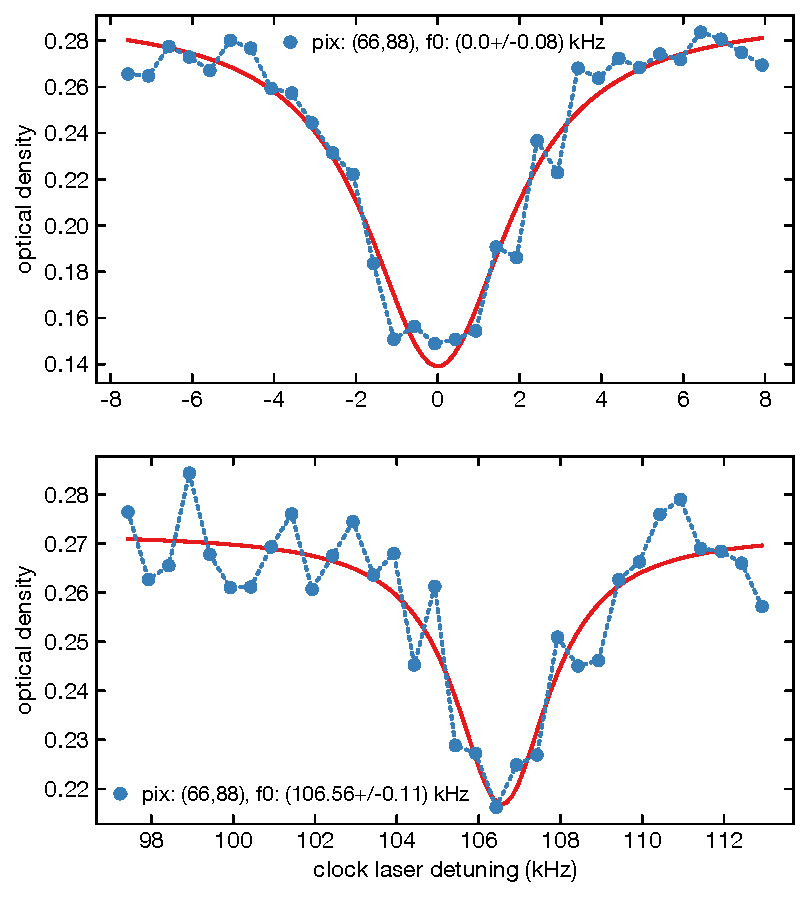
\includegraphics[scale=0.5]{figures/high_depth66_88.pdf}
				\caption{}
			\end{subfigure}
			\qquad\qquad
			\begin{subfigure}[b]{0.4\linewidth}
				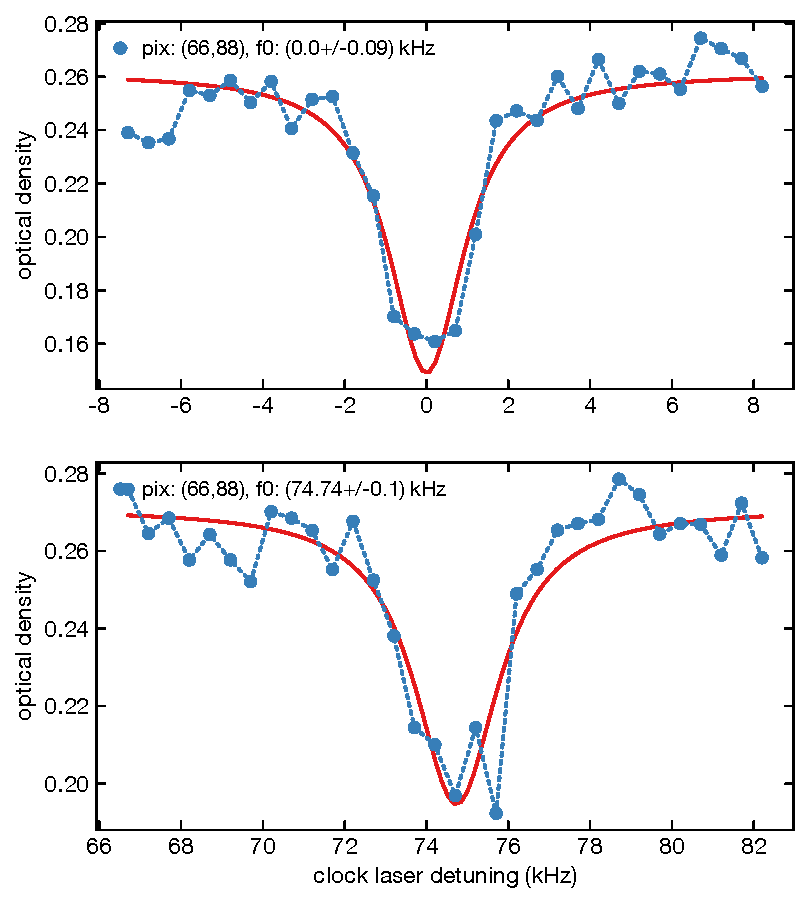
\includegraphics[scale=0.5]{figures/half_depth66_88.pdf}
				\caption{}
			\end{subfigure}

			\begin{subfigure}{\linewidth}
				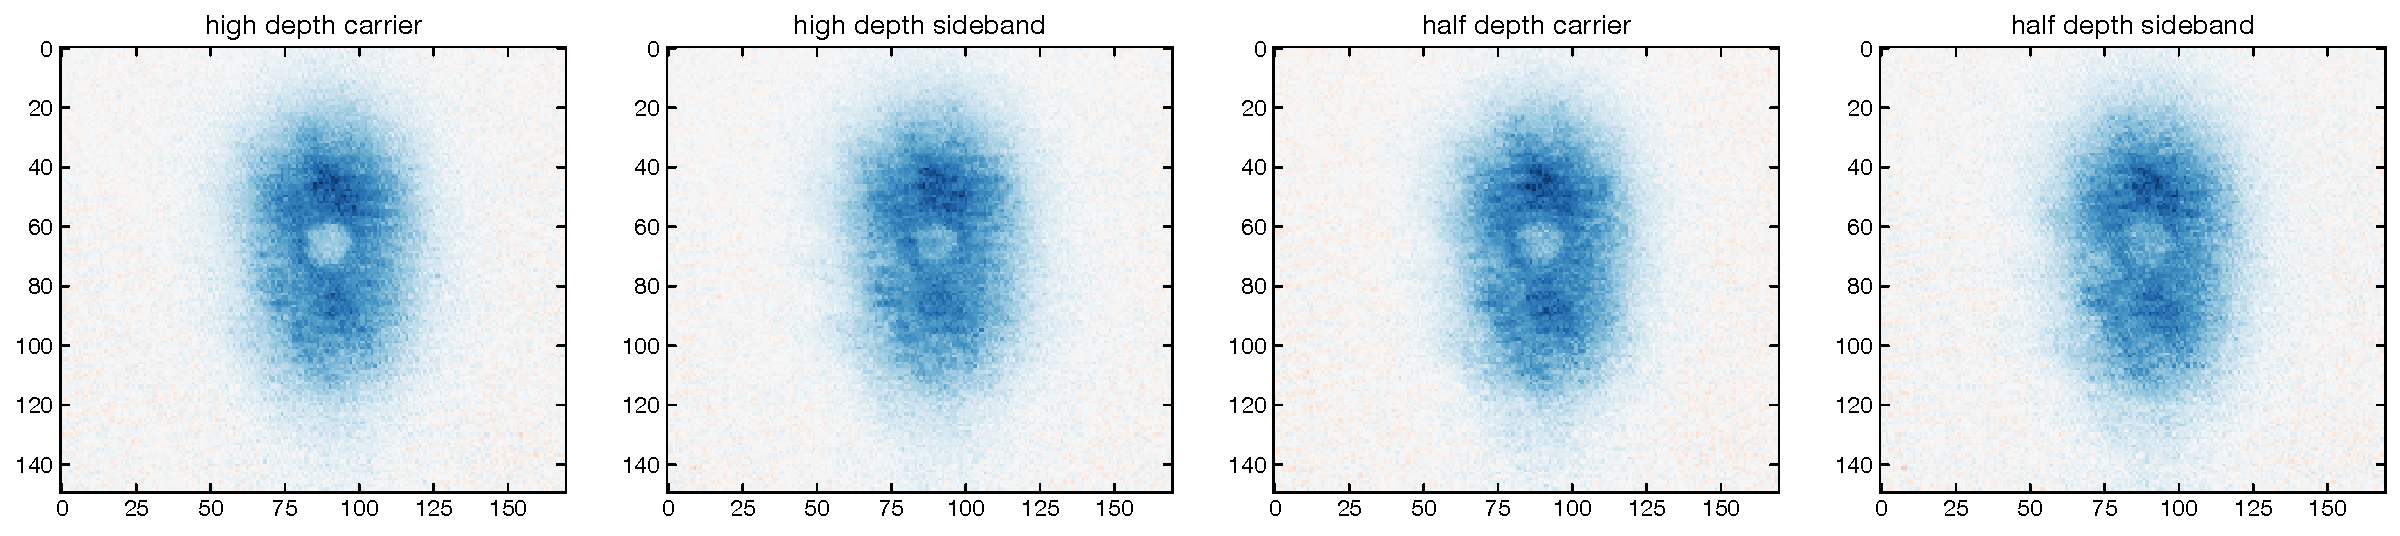
\includegraphics[scale=0.4]{figures/insitu_images.pdf}
				\caption{}
			\end{subfigure}
			\caption{\textbf{(a)} carrier (top) and sideband (bottom) clock spectra of ground and excited states of high depth \textbf{(b)} same as (a) for half of the depth \textbf{(c)} in-situ \SSZ images at the center frequency of carrier and sideband spectra (data folder: \textbackslash data \textbackslash\_2020\textbackslash12\textbackslash02\textbackslash it\_sr88\_absolute\_ac\_stark)} 
			\label{fig:total_ac_stark_spectrum}

			\end{figure}


			\noindent Quadratic zeeman shift should be an order of kHz at 50 G that was used for the measurement. 

		% The spacing between $f_{00}$ and $f_{11}$ transition is 


		% 	\begin{align*}
		% 		f_{00}-f_{11}&=(E^{e}_{0,0}-E^{g}_{0,0})/h-(E^{e}_{1,1}-E^{g}_{1,1})/h \\
		% 		&=(\nu_e-\nu_{\text{rec}}-\nu_g+\nu_{\text{rec}})-(2\nu_e-2\nu_{\text{rec}}-2\nu_g+2\nu_{\text{rec}}) \\
		% 		&=(\nu_e-\nu_g)-(2\nu_e-2\nu_g) \\
		% 		&=\nu_g-\nu_e \\
		% 	\end{align*}


		% One can also look at the spacing between the $n_{00}$ and $n_{10}$ transitions which is related to $f_{n_{00}}-f_{n_{11}}=h(\nu_{\text{g}}-\nu_{\text{e}})=h\nu_{\text{g}}(1-\sqrt{\frac{\alpha_e}{\alpha_g}})$. 



		% Alternatively, one can measure the ratio of ground and excited polarizability:

		% \begin{align*}

		% \end{align*}

	% \subsection{Waist measurements}




	% \subsection{temperature}

\section{Cross-check}
	\subsection{Discrepancies between total ac-Stark \& Trap frequency measurements}

		We compare the polarizability ratio we measured against the polarizabilities that Marianna sent us, which are (261.09 $\pm$ 1.16) a.u. at 914.0 nm and (260.91 $\pm$ 1.16) a.u. at 915.0 nm for $\alpha_g$ and (220.8 $\pm$ 2.3) a.u. for at 914.332 nm $\alpha_e$. To find out the $\alpha_g$, I linearly interpolate and get (261.03 $\pm$ 0.87) at 914.332 nm. The comparison with our measurement and Marianna's number is shown in Figure \ref{fig:ratio_comparison_plot}.

		\begin{figure}
		    % \centering
		    \hspace*{-0.5cm}
		    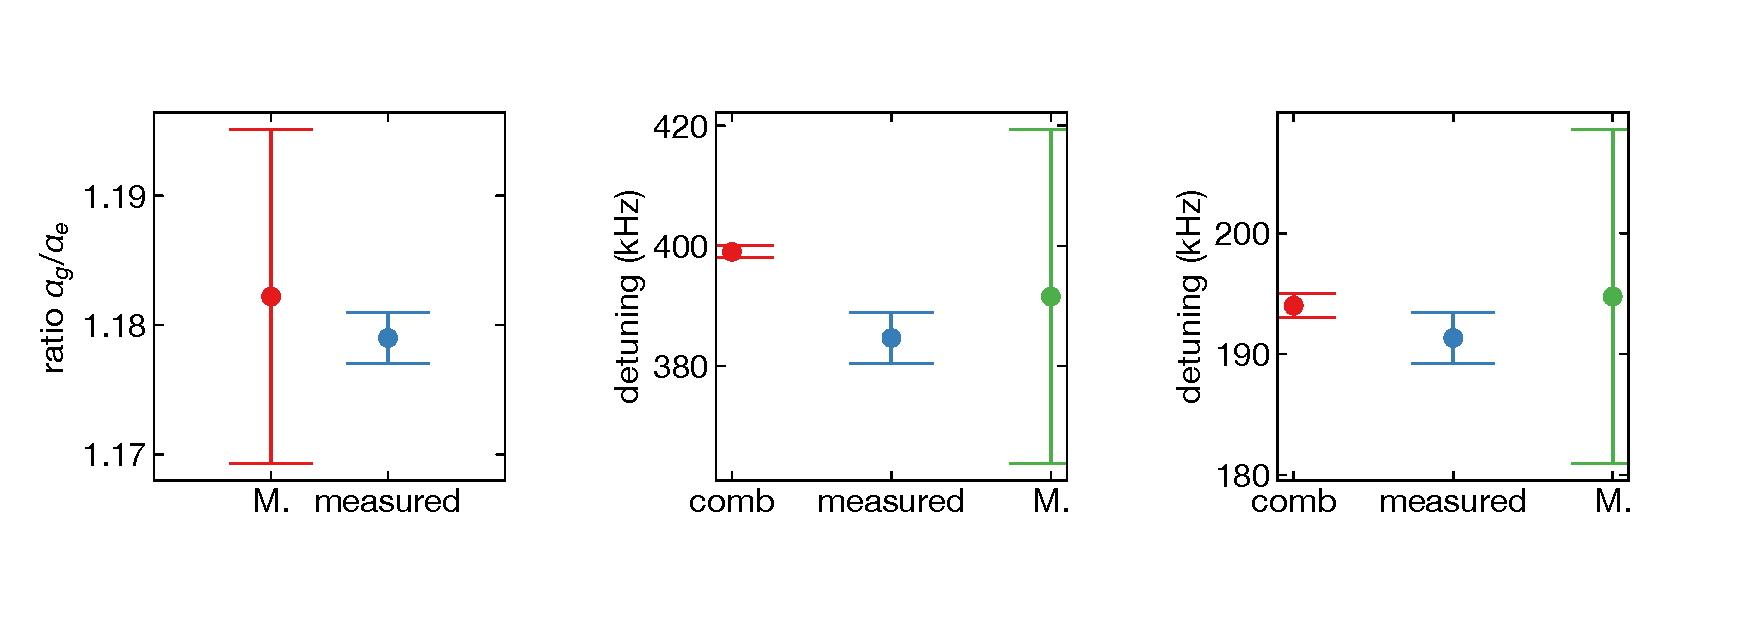
\includegraphics[scale=0.6]{figures/ratio_comparison_plot.pdf}
		    \caption{}
		    \label{fig:ratio_comparison_plot}
		\end{figure}


\section{Appendices}

\subsection{Magnetic field calibration}
		
		\begin{figure}[h]
		    \centering
		    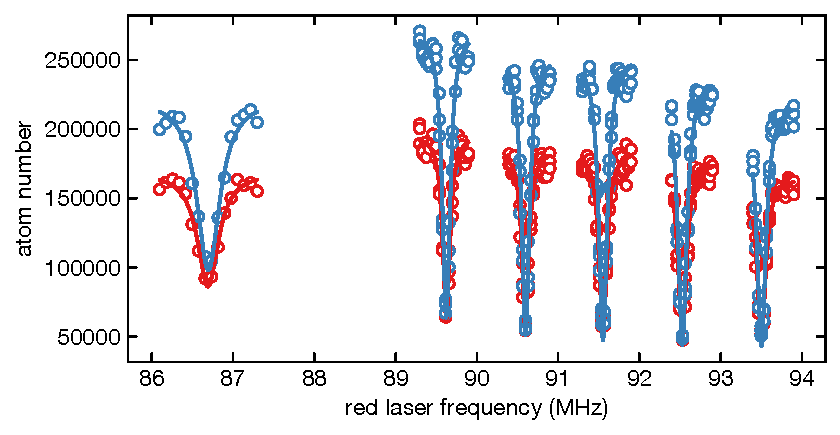
\includegraphics[scale=0.8]{figures/field_calibration.pdf}
		    \caption{\TPO m=1 transition frequency shift as a function of field set voltage datapath:\textbackslash data \textbackslash\_2020\textbackslash10\textbackslash26\textbackslash it\_field\_calibration}
		    \label{fig:field_calibration}
		\end{figure}

		\begin{figure}
		    \centering
		    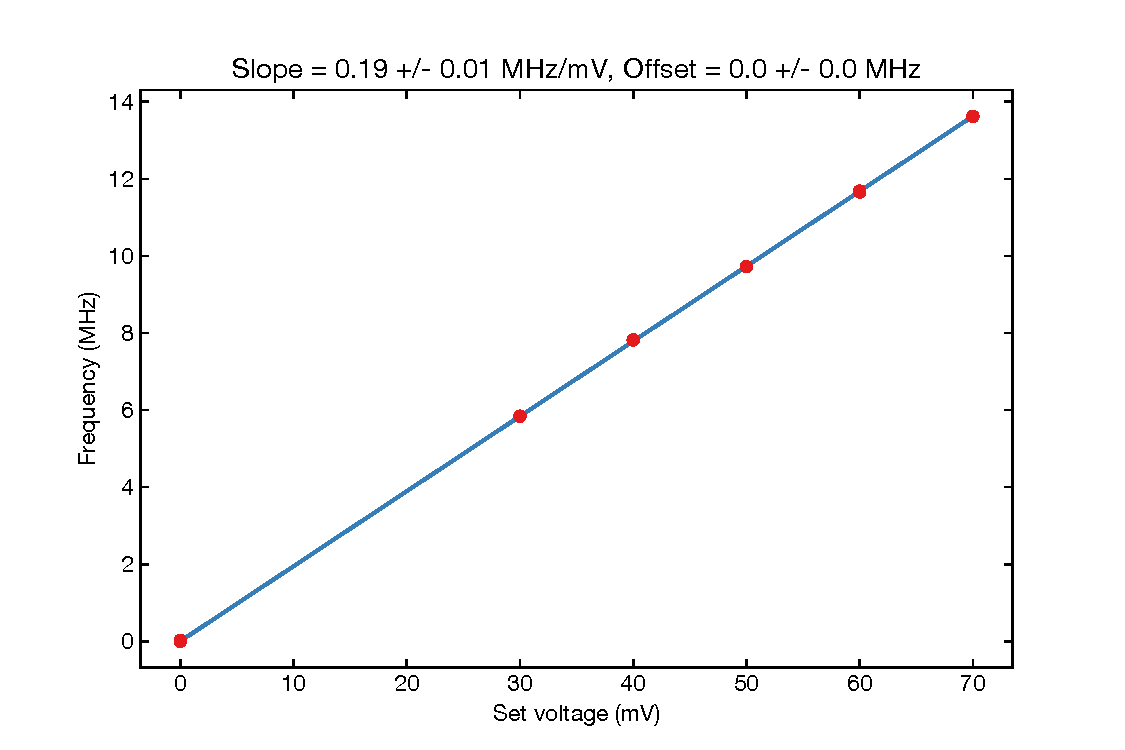
\includegraphics[scale=0.8]{figures/field_calib_curve.pdf}
		    \caption{field calibration curve}
		    \label{fig:field_calib_curve}
		\end{figure}

\subsection{Clock laser waist calibration}
\subsection{Quadratic Zeeman Shift}

		\begin{figure}
		\centering
		\label{fig:qz}
		\begin{subfigure}{0.4\linewidth}
		    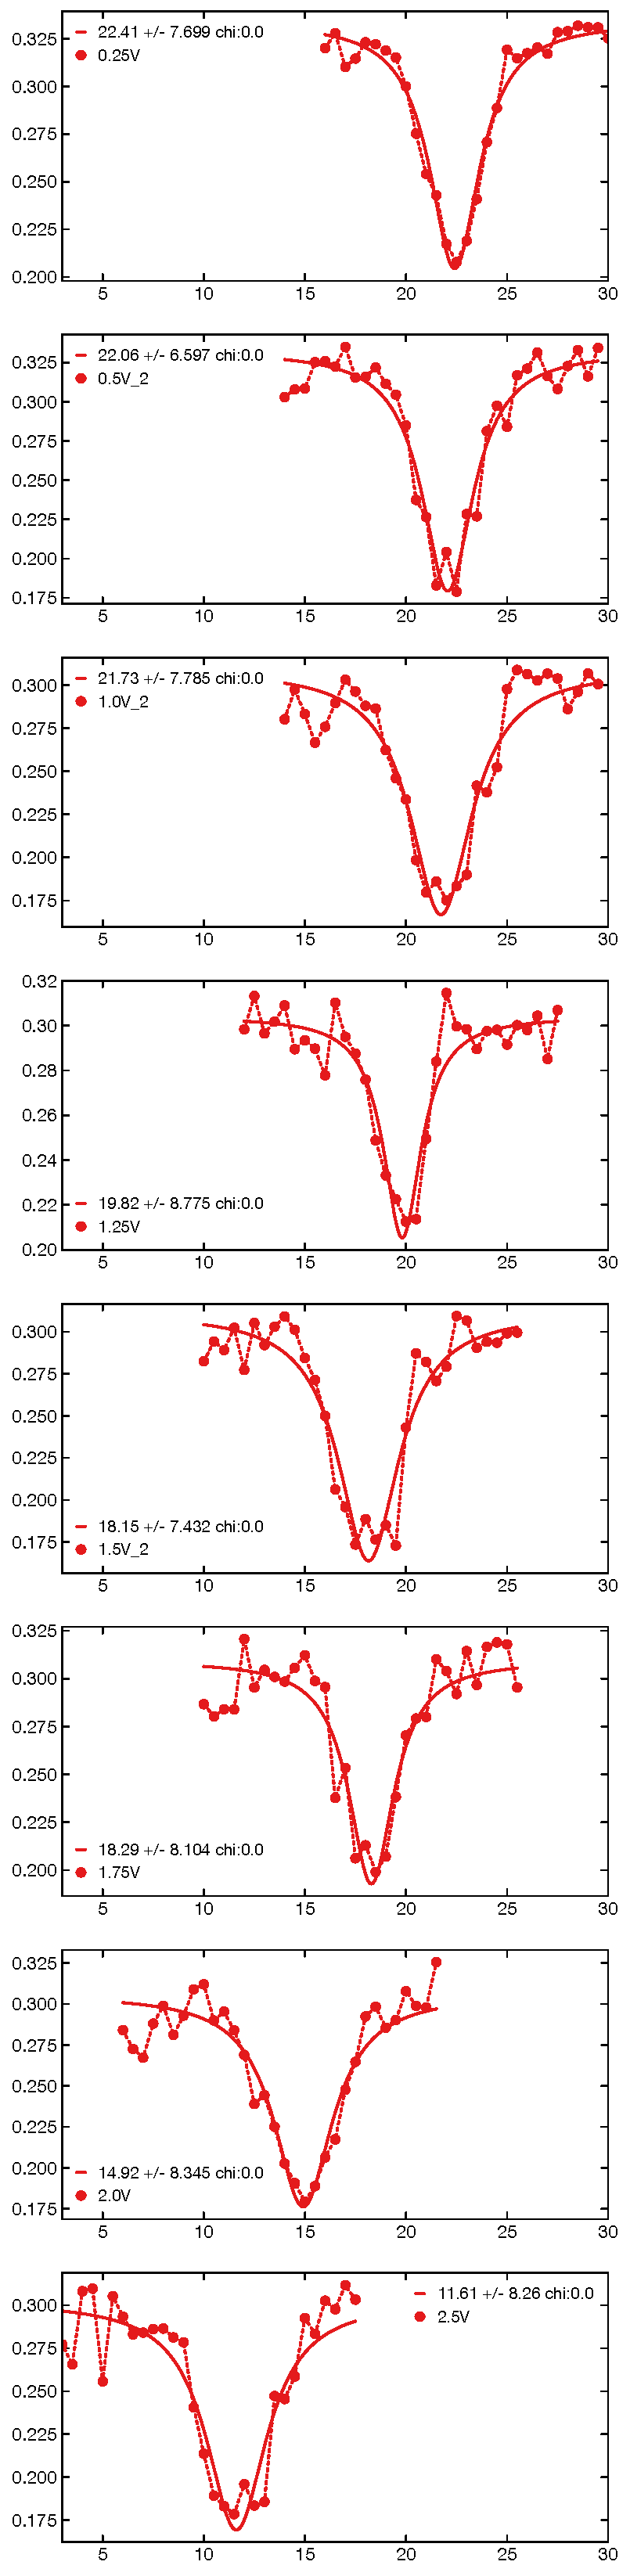
\includegraphics[scale=0.4]{figures/qz_spectrum.pdf}
		    \caption{clock resonant frequency shift for different field}
		\end{subfigure}
		\begin{subfigure}{0.4\linewidth}
		    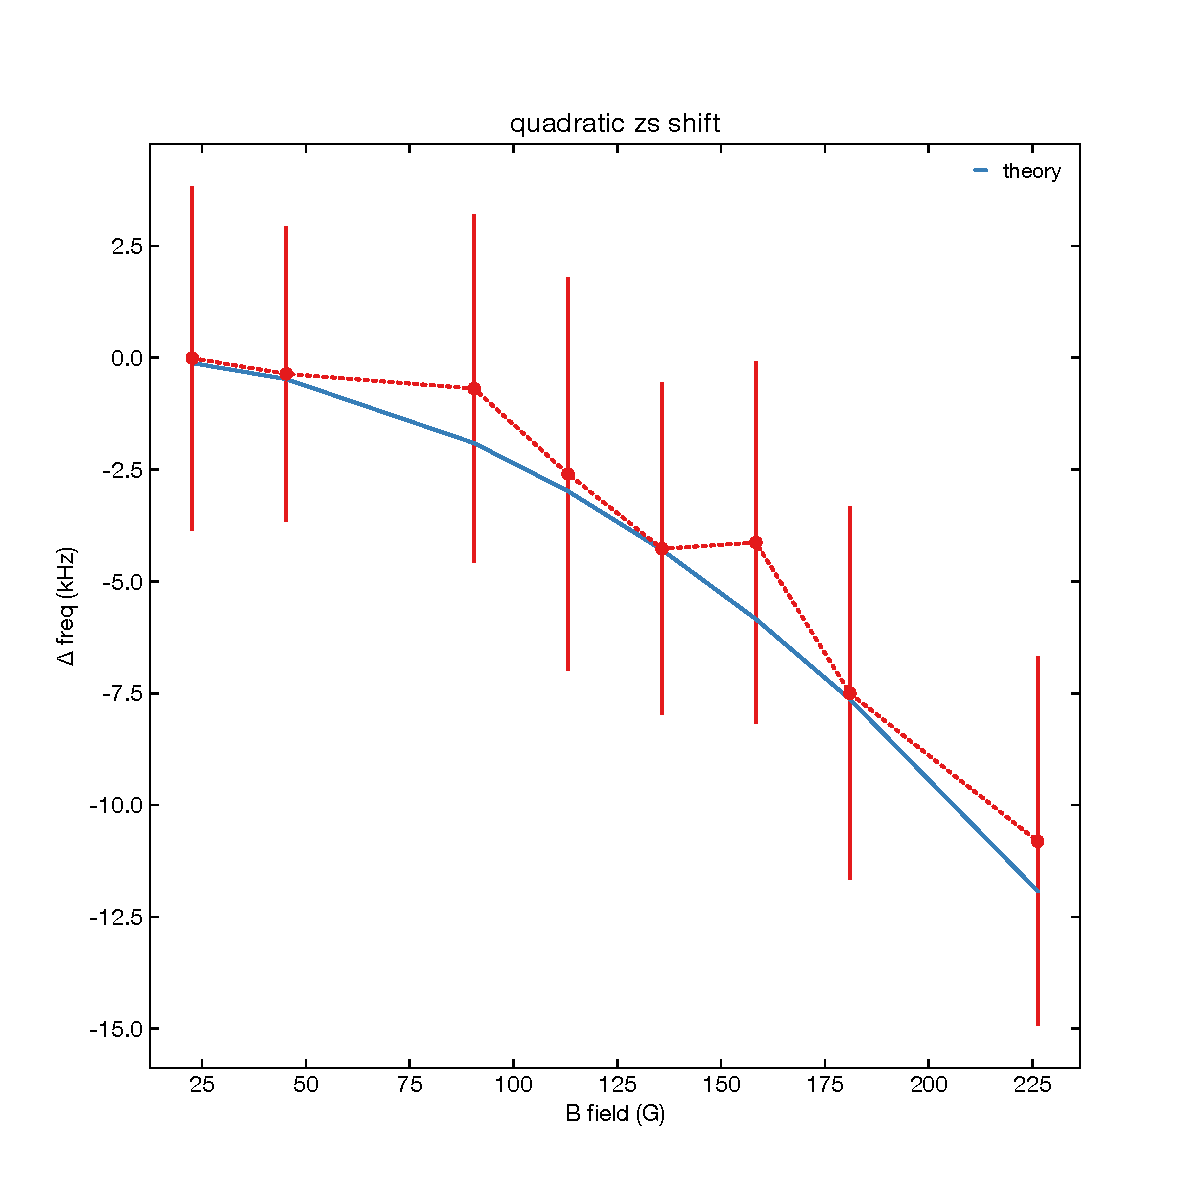
\includegraphics[scale=0.4]{figures/quadratic_zeeman_shift.pdf}
		    \caption{Quadratic zeeman shift}
		\end{subfigure}
		\caption{}
		\end{figure}


		% \begin{figure}
		% % \centering 
		% \hspace*{-2cm}
		% \label{fig:pol_ratio}
		% \begin{subfigure}{0.4\linewidth}
		% 	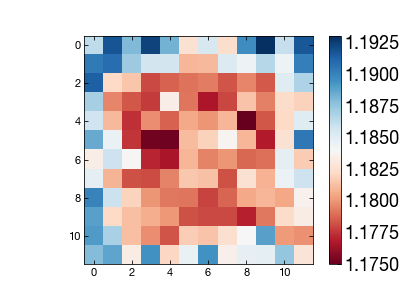
\includegraphics[scale=0.7]{figures/pol_ratio_size6.png}
		% 	% \caption{}
		% \end{subfigure}
		% \qquad\qquad\qquad\quad
		% \begin{subfigure}{0.4\linewidth}
		% 	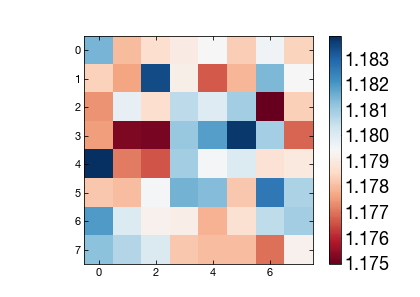
\includegraphics[scale=0.7]{figures/pol_ratio_size4.png}
		% 	% \caption{}
		% \end{subfigure}
		% \caption{Polarizability $\alpha_g/\alpha_e$ ratio for (a) larger size (b) smaller size} 
		% \end{figure}

			% \begin{figure}
			% \centering 
			% \begin{subfigure}[b]{0.4\linewidth}
			% 	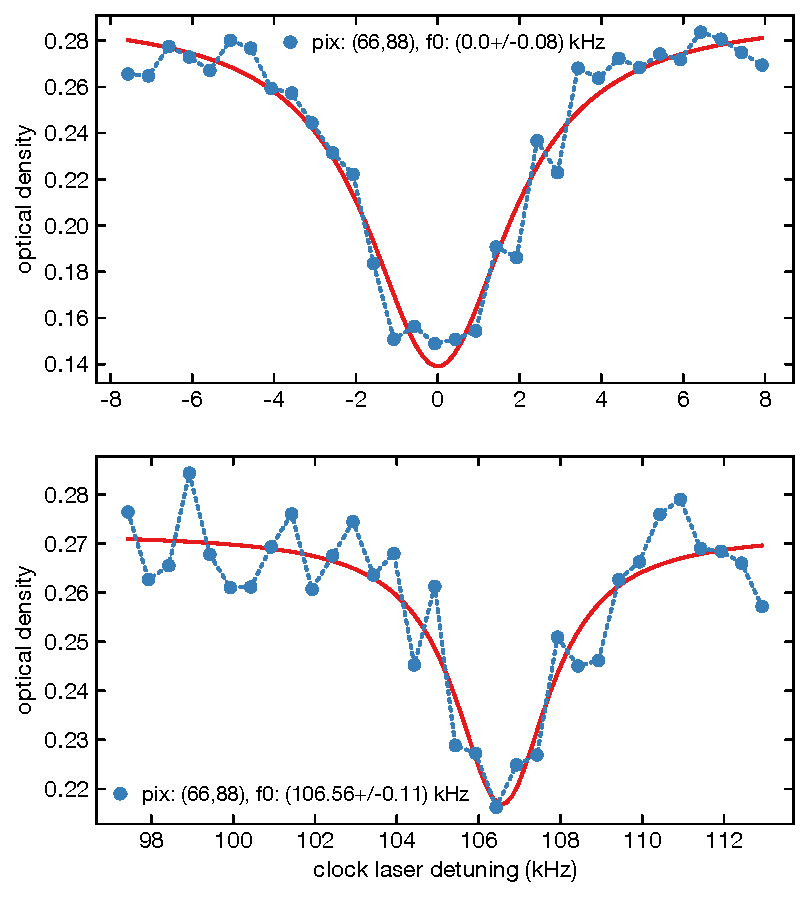
\includegraphics[scale=0.5]{figures/high_depth66_88.pdf}
			% 	\caption{}
			% \end{subfigure}
			% \qquad\qquad
			% \begin{subfigure}[b]{0.4\linewidth}
			% 	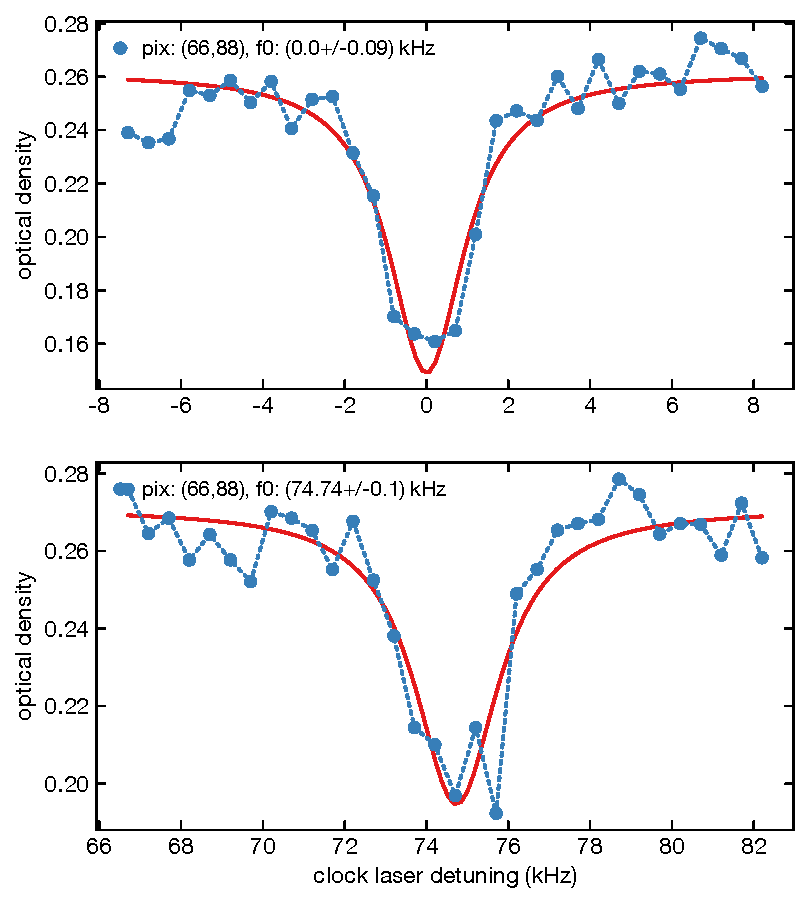
\includegraphics[scale=0.5]{figures/half_depth66_88.pdf}
			% 	\caption{}
			% \end{subfigure}

			% \begin{subfigure}{\linewidth}
			% 	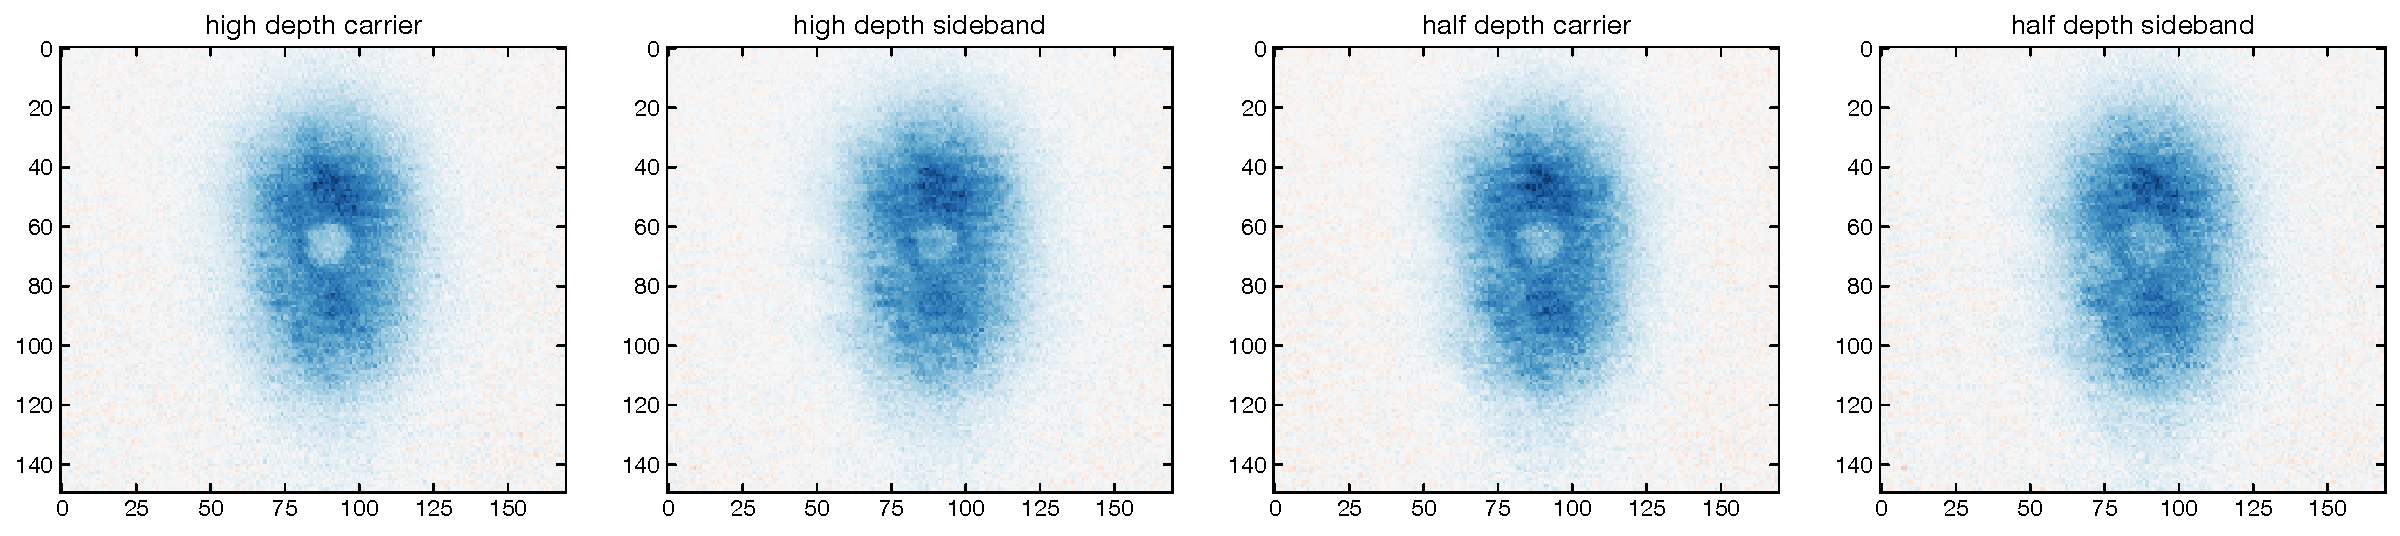
\includegraphics[scale=0.4]{figures/insitu_images.pdf}
			% 	\caption{}
			% \end{subfigure}
			% \caption{\textbf{(a)} carrier (top) and sideband (bottom) clock spectra of ground and excited states of high depth \textbf{(b)} same as (a) for half of the depth \textbf{(c)} in-situ \SSZ images at the center frequency of carrier and sideband spectra (data folder: \textbackslash data \textbackslash\_2020\textbackslash12\textbackslash02\textbackslash it\_sr88\_absolute\_ac\_stark)} 
			% \label{fig:total_ac_stark_spectrum}

			% \end{figure}


\subsection{Ac-Stark shift from the clock laser}
	very small
% \subsection{Magnetic field calibration}
% \subsection{Probe intensity calibration}

\bibliography{main}{}
\bibliographystyle{plain}

\end{document}
